\section{AMIDST model class}

%\textcolor{red}{OUt-of-topic: Shouldn't we use Figure numbering based on section? The deliverable is expanding like the universe...}\\

One of the main goals of AMIDST project is the definition of a general model class with the following characteristics: 

\begin{itemize}
\item \textbf{Feature 1:} It should be applicable to the three considered use-cases, i.e., Daimler, Cajamar, and Verdande,

\item \textbf{Feature 2:} it should be scalable, supporting both inference and learning from massive data streams and

\item \textbf{Feature 3:}  it should be general enough to be applicable to any future, potentially similar, use-cases.

\end{itemize}

Taking these different characteristics into account and using the subnetwork graphical notation introduced in Section \ref{SubSection:GraphicalNotation}), we will first present and discuss the general AMIDST model class in Section \ref{GeneralModelClass}, then its specific instantiation to each use-case in different subsections. Finally, a summary is presented in Section \ref{summaryAMIDSTModels}.

%---------------------------------------------------------------------
\subsection{The general AMIDST model class}\label{GeneralModelClass}
%---------------------------------------------------------------------

Figure \ref{Figure:AMIDSTModelClass} shows the proposed general AMIDST model class. This model is the result of combining all the models required by the different problem domains above presented. In order to find the commonalities between all models, higher-level descriptors have been required to reinterpret the individual models, that is, instead of all the individual variables, subnetworks have been used to group variables with similar properties.


\begin{figure}[ht!]
\begin{center}
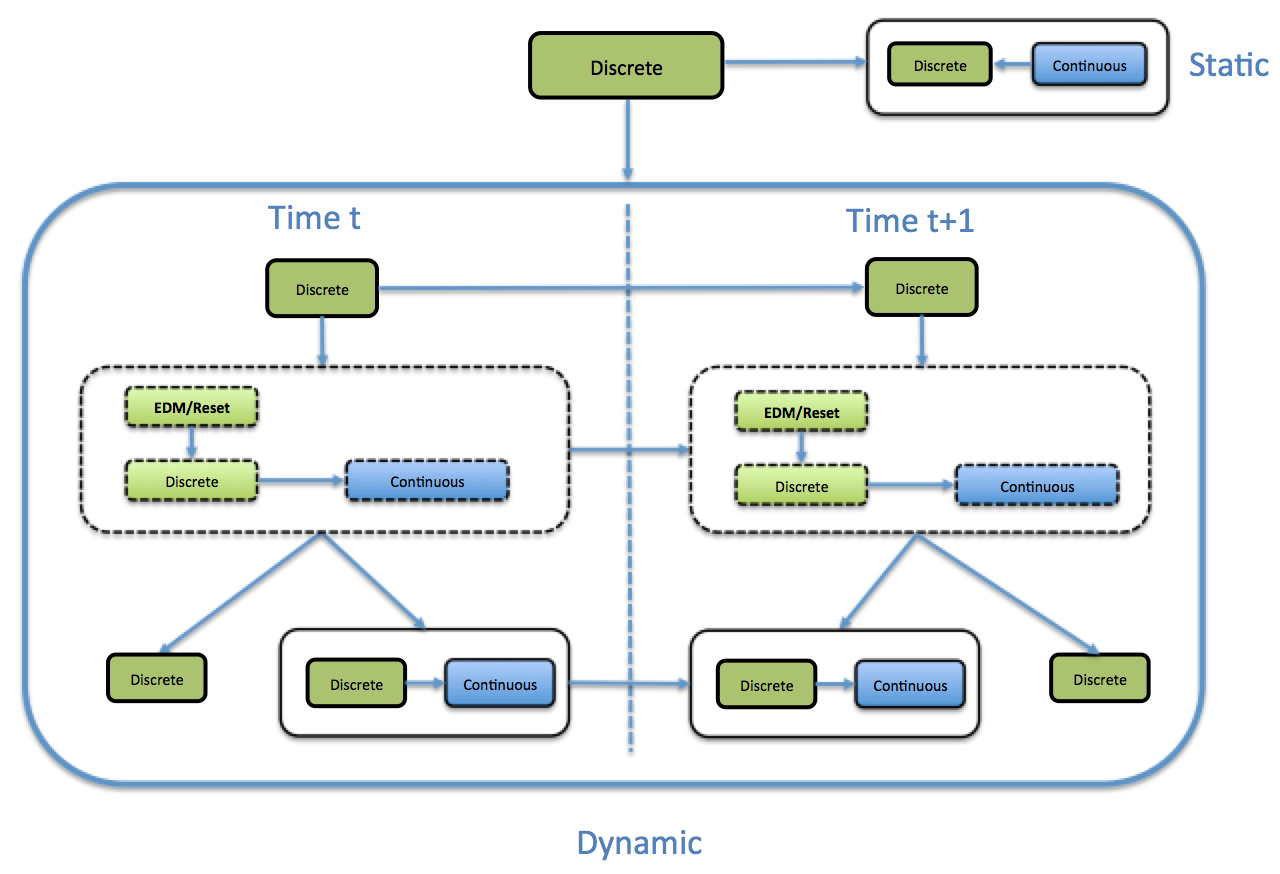
\includegraphics[scale=0.465]{./figures/AMIDSTModelClass}
\caption{\label{Figure:AMIDSTModelClass} Proposed AMIDST model class.}
\end{center}
\end{figure}


This model class can be seen as a 2T-DBN, i.e. it satisfies the first order Markov property and the stationary assumption. However, this model is not as general as 2T-DBN and contains much more internal structure. More precisely, the structure of this model decomposes along 3 main different layers which can be described are follows:

\begin{itemize}

\item \textbf{Control/class layer:} The upper layer corresponds to a subnetwork of either discrete or continuous observed variables, that would generally act as control continuous variables or the class variable. Variables can be connected through consecutive time steps to encode temporal dependences, e.g. the probability of a particular class label at time $t$ varies with respect to the label at time $t-1$. Existing links from continuous observed links to state variables in the lower layer, will be possibly handled with logit and probit functions.

\item \textbf{Hidden layer:}  The second layer corresponds to a set of interconnected discrete and continuous hidden variables, for which only links from discrete to continuous nodes are allowed. We will use the term \textit{state} variables to denote the discrete ones and the term \textit{latent}\footnote{The term \textit{latent} for variables, is generally used in statistics to refer to hidden variables, as opposed to observed ones. However we will use it here to refer exclusively to continuous hidden variables.} to denote continuous variables. This layer can contain state hidden variables that are not connected over time and that could be used, for instance, to model mixture of Gaussian distributions for the observed continuous nodes they point to in the immediate lower layer. State and latent variables that are connected over time can be used to model a process that is evolving over time. Note that links from latent variables to state variables are explicitly not allowed.

\item \textbf{Observable layer:} Finally, the bottom layer corresponds to a set of interconnected discrete and continuous observed variables. Although in principle, there exist no restrictions with respect to the direction of the links, only links from discrete to continuous nodes are required by our use cases. It is possible to alleviate the sensor Markov assumption by including links between observed variables at consecutive time steps.

\end{itemize} 


In the following sections, we will reason out how each particular use case fits in this global model. In that way, we will show how this model class satisfies \textbf{Feature 1}. Our assumption is that, in a similar way, this model class can be instantiated to other related problems and fulfills \textbf{Feature 3}. So, this process of instantiating this model class to the three use-cases (all of them with different application scenarios) should also be seen as pedagogical examples showing the potential applicability of this subclass of 2T-DBNs. The remaining task is to design inference and learning algorithms that allow the application of this model family to massive data streams. 


%---------------------------------------------------------------------
%\subsection{The model classes of the three use-cases} \label{UseCaseModelClasses}
%---------------------------------------------------------------------

%---------------------------------------------------------------------
\subsubsection{Daimler model class}\label{daimlerAMIDSTModels}
%---------------------------------------------------------------------


Daimler's resulting model has been previously displayed in Figure \ref{Figure:daimlerLEdynGeneric}. With respect to the general model above described, we need the following concepts:

\begin{itemize}
\item \textbf{Control/class layer}: is not used in this domain.

\item \textbf{Hidden layer}: the two sets of state variables are required here. The lower set of state variables (State 2) encode a polytree \cite{JensenNielsen2007} for the hierarchy of hypothesis. This polytree structure, not explicitly encoded in the model, can indeed be exploited during inference.


Connection through time is only made at the level of top sets of state variables (``State 1''), i.e., the signal real values (S\_REAL \footnote{Although these variables are inherently continuous, we notice that they are discretized to avoid the inference problems derived of having continuous parents with discrete children (see Section \ref{Section:DaimlerDynamic}).}). Consequently, the future and past time slices of our 2T-DBN are conditionally independent given the S\_REAL variables corresponding to the present time. Additionally, inside a time slice, the observed continuous and discrete subnetworks are also conditionally independent given these S\_REAL variables. In the case that we wanted to contemplate a possible extension in which the lower level hypothesis are connected over time, then the ``State 1'' sub-networks of the model class would contain the S\_REAL variables and the temporally linked hypothesis. Although, as commented before, this would greatly difficult the inference process. 

\item \textbf{Observable layer:} there are two sets of observed variables in this case. On one hand, we encounter a group of variables representing the measured data (S\_MEAS), along with the variables encoding the sensor noise (S\_SIGMA). The resulting structure is again a polytree, with presents some advantages for the inference process. On the other hand, we have a single discrete node for the manoeuvre event, which will be the target variable during inference. 
\end{itemize}


\begin{figure}[ht!]
\begin{center}
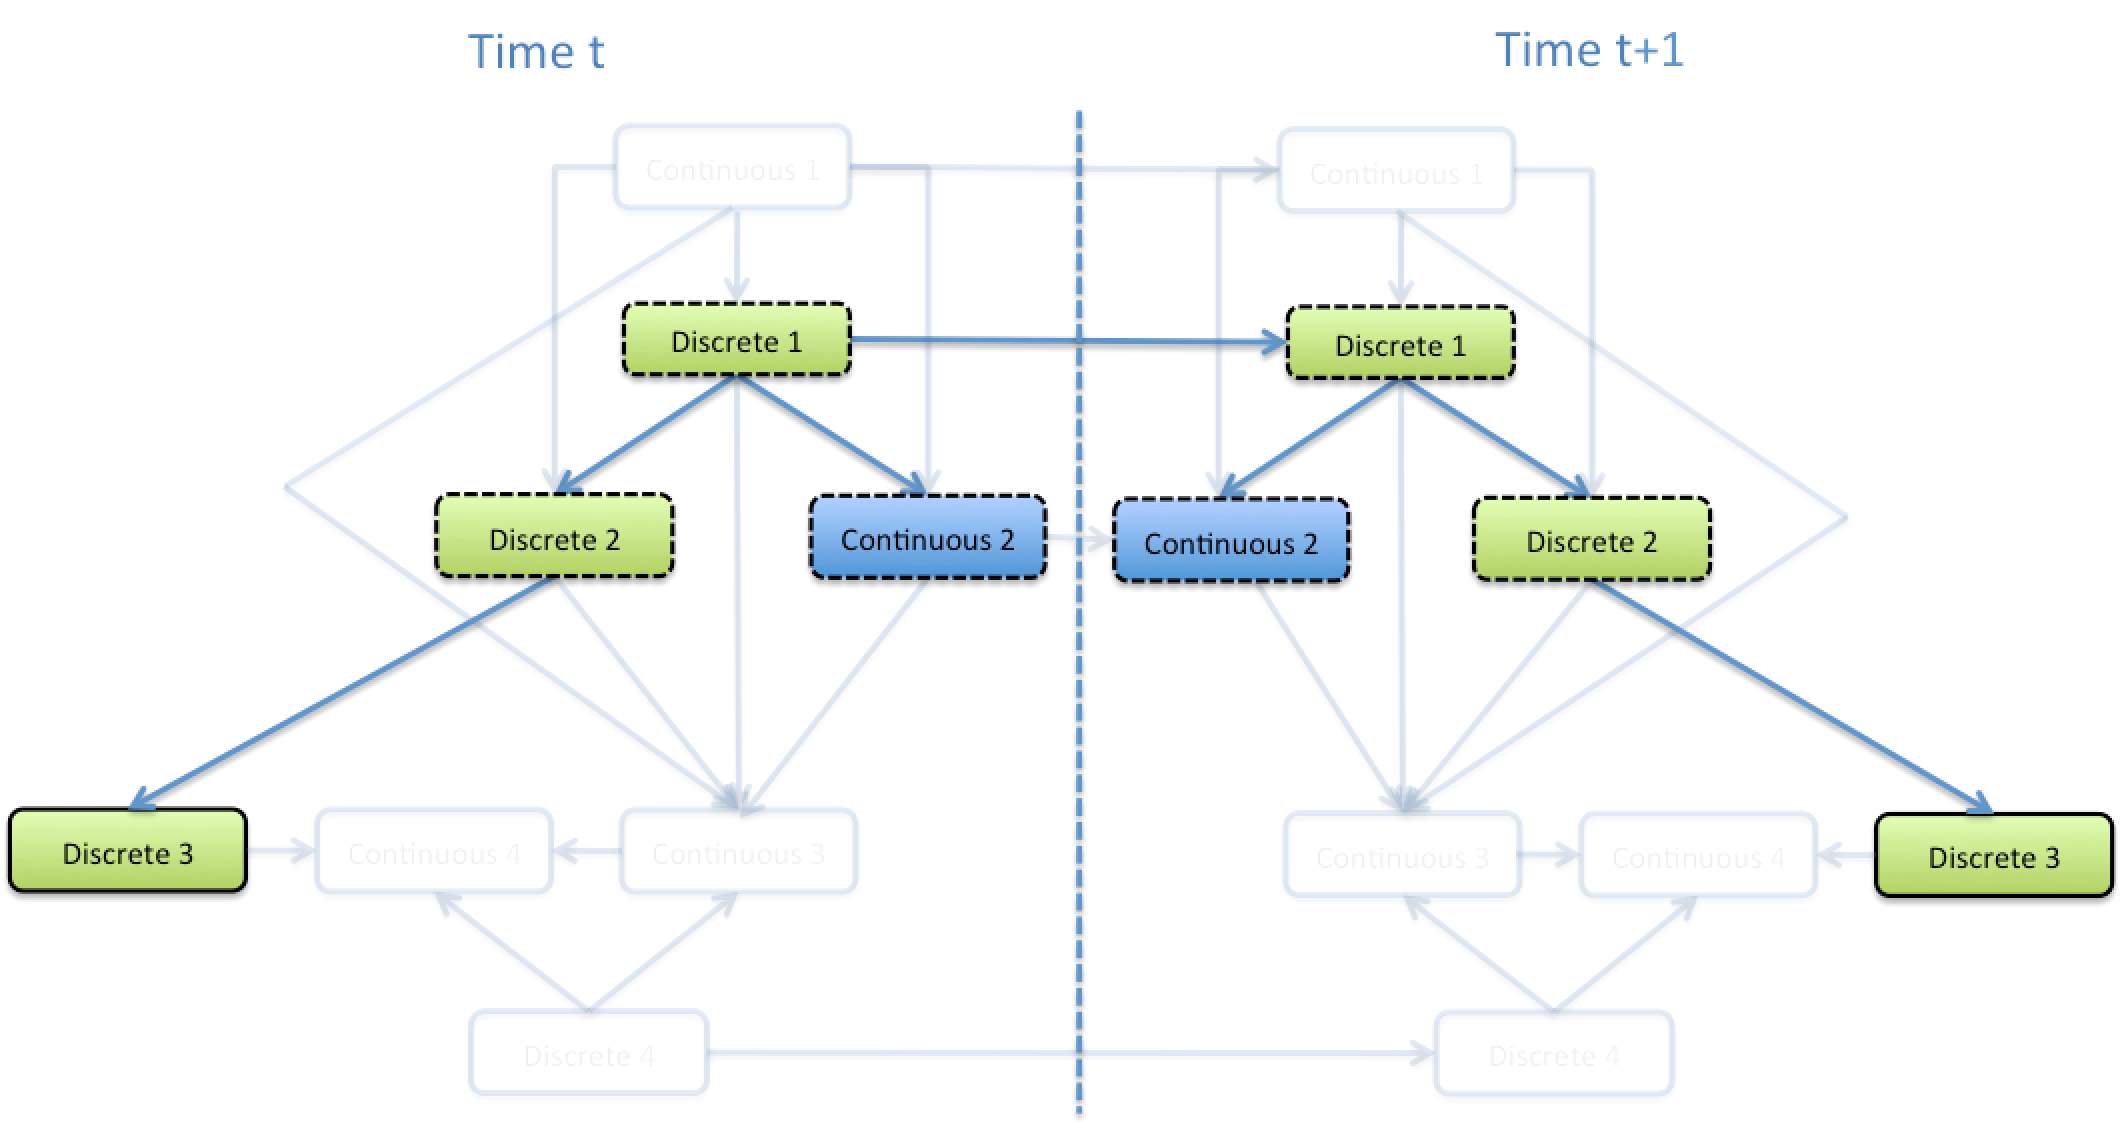
\includegraphics[scale=0.39]{./figures/AMIDSTModelClassDaimler}
\caption{\label{Figure:AMIDSTModelClassDaimler} AMIDST model class - Daimler}
\end{center}
\end{figure}

%As commented in Section \ref{Section:DaimlerDynamic}, one the main issues of this model is that it contains discrete children with continuous parents, and hence cannot be modelled with the conditional linear Gaussian family \cite{JensenNielsen2007}. In this particular case, to deal with this problem we adopt the same solution adopted in \cite{kasper2012object}, which consists in discretizing these nodes. In this way, the general structure of Daimler's models corresponds to the one depicted in Figure \ref{Figure:DaimlerModelClass}, where there is no more discrete children with continuous parents, and it is possible thereby to use standard parametrizations \cite{JensenNielsen2007}. 


%This general model is structured as a 2T-DBN (see Section \ref{SubSubSection:2DBNs}). The static model which is repeated over time consists of four elements: 
%
%\begin{enumerate}
%\item ``Discrete 1'': is a discrete hidden subnetwork which is the only element temporally connected
%\item ``Discrete 2'': is an additional discrete hidden subnetwork which is not temporally connected. It is included only for modelling purposes inside a time slice
%\item ``Discrete 3'': is an observed discrete subnetwork directly depending on ``Discrete 2'' subnetwork
%\item  ``Continuous 1'': is an observed continuous subnetwork which is directly depending on ``Discrete 1'' subnetwork
%\end{enumerate}
%
%As commented, this 2T-DBN is only temporally connected through the hidden subnetwork on top. 



%---------------------------------------------------------------------
\subsubsection{CajaMar model class}\label{cajamarAMIDSTModels}
%---------------------------------------------------------------------
%\textcolor{blue}{To be re-written}
Concerning CajaMar use-case, both application scenarios share the same models, of which two versions have been previously discussed, namely, static and dynamic (see Section \ref{Section:CajaMarModels}). 

At this point, we obviate the static version, because the general AMIDST model class is primarily a dynamic model class. Therefore, the high-level description of CajaMar's dynamic model (previously displyed in Figure \ref{fig:component}) is given in Figure \ref{Figure:AMIDSTModelClassCajamar}. %As it can be seen, CajaMar models is composed by four main subnetworks, which are expanded over time and all of them are observed. Hence, at CajaMar, there are no hidden subnetworks. 


\begin{figure}[ht!]
\begin{center}
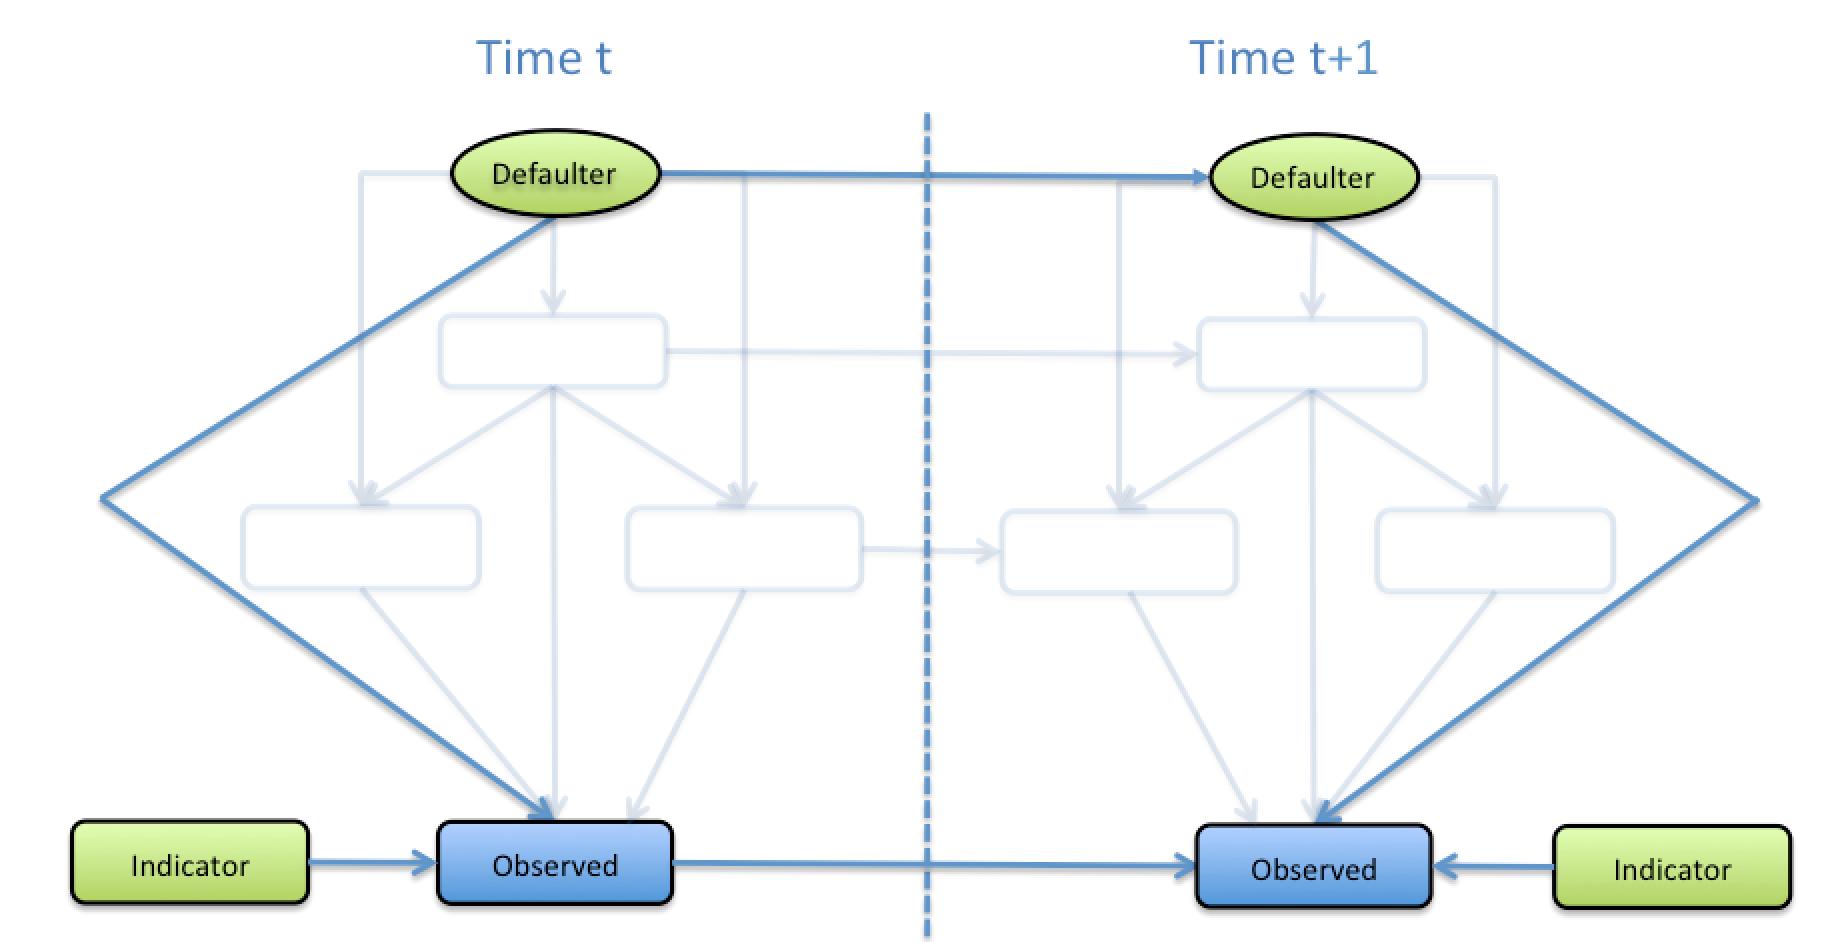
\includegraphics[scale=0.39]{./figures/AMIDSTModelClassCajamar.png}
\caption{\label{Figure:AMIDSTModelClassCajamar} AMIDST model class - Cajamar.}
\end{center}
\end{figure}


Following the layer-wise analysis used above, Cajamar's model is described as:
\begin{itemize}

\item \textbf{Control/class layer}: the top node ``Defaulter" in this layer represents the class variable to categorize a client as defaulter or non-defaulter. There exist temporal links between consecutive time steps to model the dynamic nature of being a defaulter or non-defaulter. Note that this is indeed the target variable in the inference process.

\item \textbf{Hidden layer}: is not used in this domain.

\item \textbf{Observable layer:} The ``Observed" continuous subnetwork represents information corresponding to the socio demographics, memory variables, financial activity and past payment behaviour of a client, which in principle may or may not be connected over time. The ``Indicator" subnetwork, in turn, comprises the set of indicator variables, $\delta_{X_t}$, used to model the situation in which one of the continuous variables has a large number of zeroes.

\end{itemize}



%---------------------------------------------------------------------
\subsubsection{Verdande model class}\label{verdandeAMIDSTModels}
%---------------------------------------------------------------------

Figure \ref{Figure:AMIDSTModelClassVerdande} shows how the general AMIDST model class is instantiated in the case of Verdande. This instantiated model encompasses the models of the three applications scenarios detailed in Figures \ref{Figure:VTScenario1}, \ref{Figure:VTScenario2} and \ref{Figure:VTScenario3}  (see Section \ref{Section:VerdandeModels}).  We now comment the main elements of this instantiated model.


\begin{itemize}
\item \textbf{Control/class layer}:  This element is instantiated to a set of nodes modelling the observed control variables. In the three application scenarios, the role of this control variables is to condition the transition probability of the state variables and allow the modelling of non-stationary transition probabilities.  

\item \textbf{Hidden layer}: This element is directly instantiated from the general class. However, there are some differences when applied to each particular application scenario. For the first application scenario (see Figure \ref{Figure:VTScenario1}),  ``State 2'' is not needed and ``State 1'' is instantiated to the ``Normal/Abnormal'' state variable. For the second application scenario, ``State 1'' is no needed and ``State 2'' is instantiated to a single multinomial variable whose role is to model mixture of Gaussians at the leaves. In the third application scenario, ``State 2'' is no used and ``State 1'' is instantiated to a sub-network containing the FormationDetection and Switch nodes. 

\item \textbf{Observable layer: } This element of the model class is similarly instantiated in the three application scenarios. In the case of application scenario 1 and 3, it is just instantiated to a single response variable. In the application scenario 2, this instantiation can be made over a set of (possibly interconnected) response variables. 
\end{itemize}



\begin{figure}[ht!]
\begin{center}
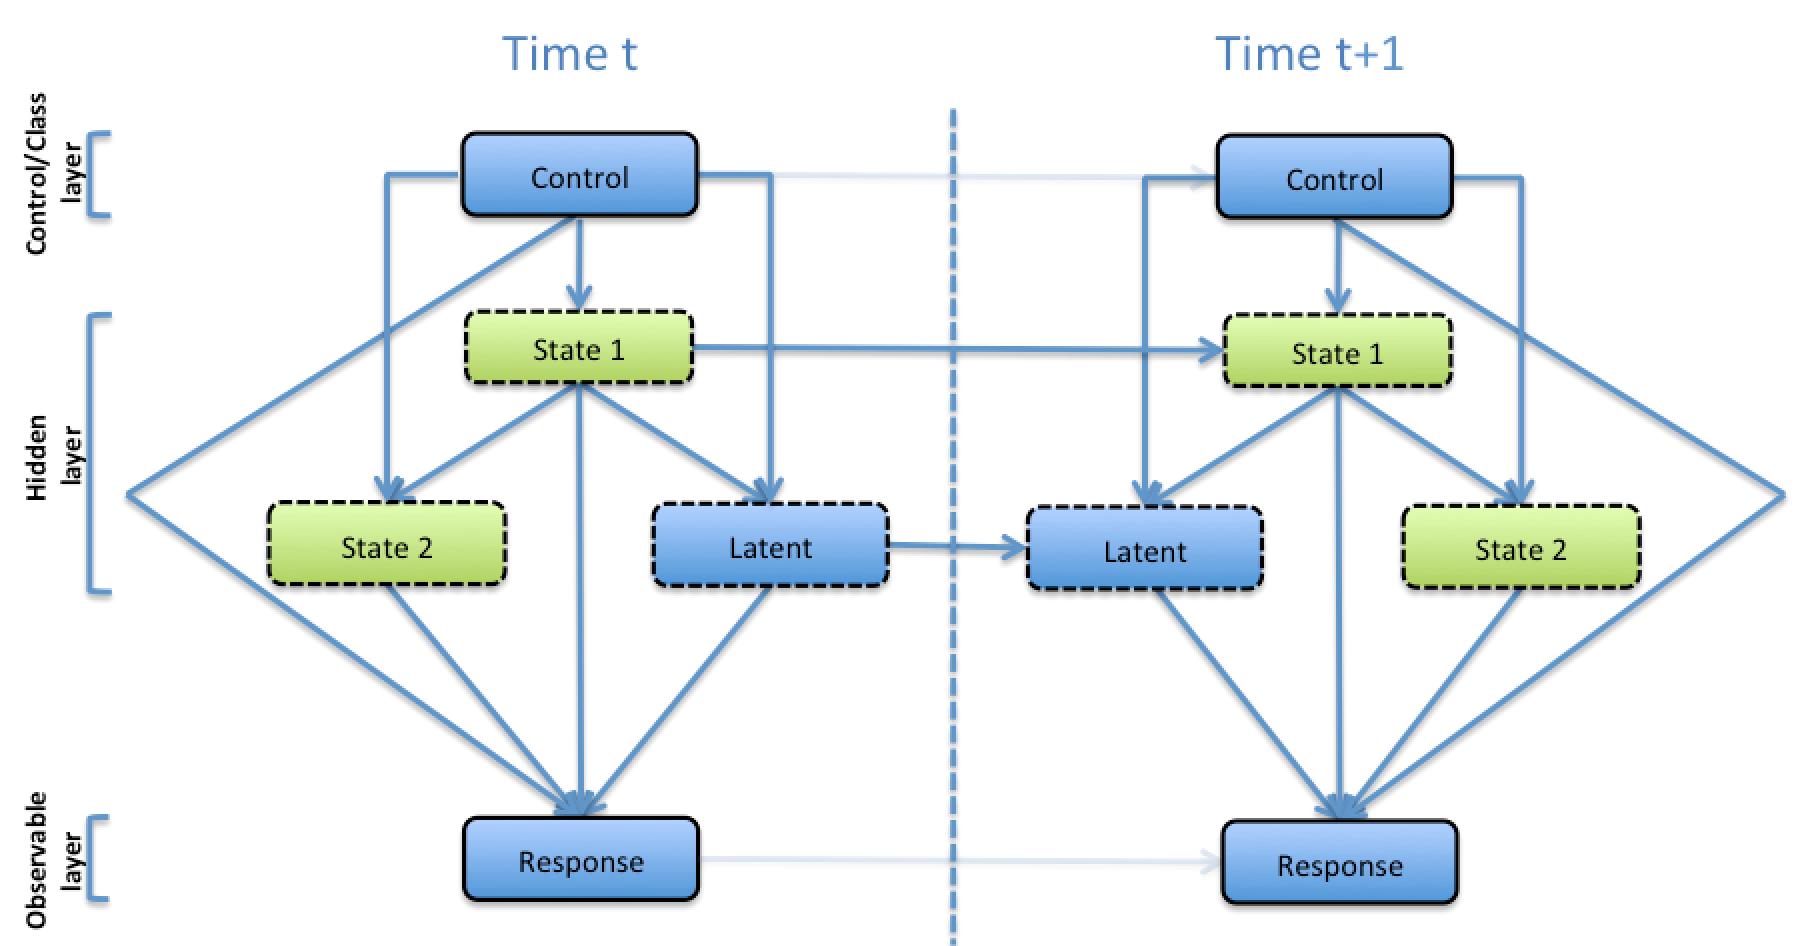
\includegraphics[scale=0.39]{./figures/AMIDSTModelClassVerdande}
\caption{\label{Figure:AMIDSTModelClassVerdande} AMIDST model class - Verdande.}
\end{center}
\end{figure}


\subsection{Summary}\label{summaryAMIDSTModels}

As it has been shown in the previous sections, the proposed AMIDST model class of Figure \ref{Figure:AMIDSTModelClass} encompasses the different application scenarios of the three use cases. These three use-cases come from very different domains: automotive, finance and oil-drilling. In our opinion, these are strong arguments in favour of the generality and applicability of this model class. Although, in any case, a better understanding of the faced problems and/or future applications might reveal that some elements of this model class need to be refined.  

A higher level view of our proposed AMIDST model is displayed in Figure \ref{Figure:AMIDSTModelClassHighLevel}, that could actually be seen as a ``restricted" 2T-DBN, which is restricted in the sense that continuous hidden variables cannot point to discrete nodes. In this model, the three above-described layers are clearly represented. Broadly speaking, the \textit{control/class layer} represent control variables that may affect the process homogeneity/stationarity, or represent the class variable in classification tasks; the \textit{hidden layer} includes a sufficiently rich set of hidden variables to capture the process dynamics; finally, the \textit{observable layer} encompasses sensor measures and predictive attributes. We believe that proper instantiation of these three layers will allow to apply the AMIDST model to a wide range of use case domains.

%A representation of this higher level of abstraction is shown in Figure \ref{Figure:AMIDSTModelClassHighLevel}. \textcolor{red}{Add layer names to Figure \ref{Figure:AMIDSTModelClassHighLevel}}

\begin{figure}[ht!]
\begin{center}
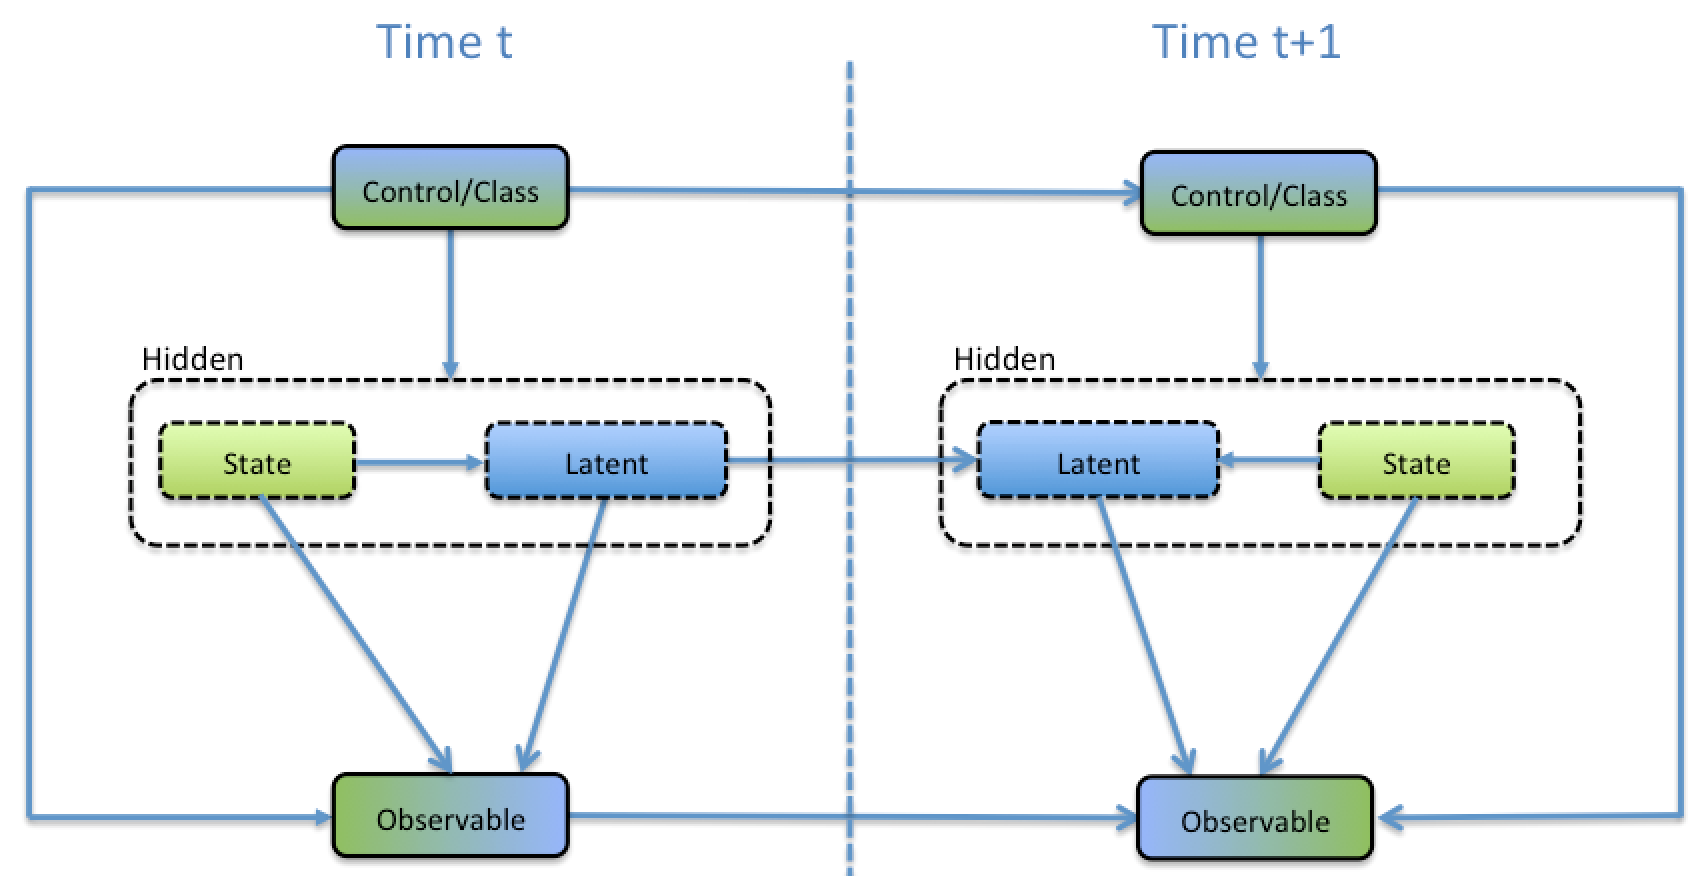
\includegraphics[scale=0.4]{./figures/AMIDSTModelClassGeneral}
\caption{\label{Figure:AMIDSTModelClassHighLevel} The high-level AMIDST model class}
\end{center}
\end{figure}


%This section, with the high-level figure, should help to defend the third point made in the introduction, i.e., that it should be general enough to be applicable to any future, potentially similar, use-cases.
 


%\begin{figure}[ht!]
%\begin{center}
%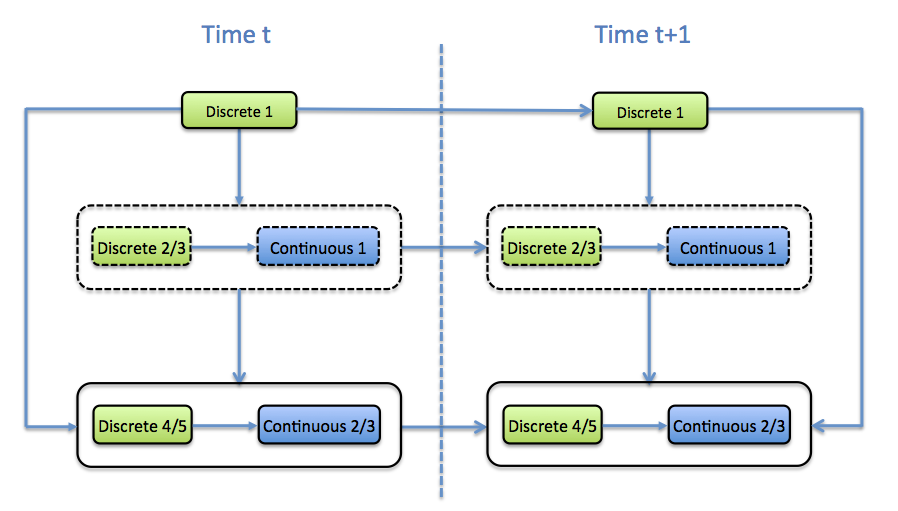
\includegraphics[scale=0.4]{./figures/AMIDSTModelClassHighLevel}
%\caption{\label{Figure:AMIDSTModelClassHighLevel} AMIDST model class high level}
%\end{center}
%\end{figure}

%\begin{figure}[ht!]
%\begin{center}
%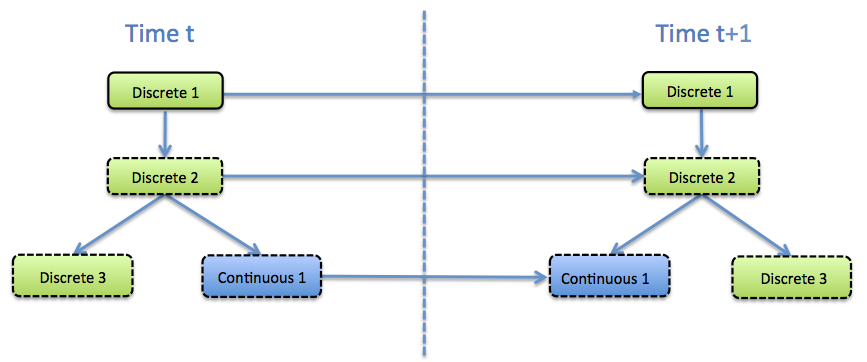
\includegraphics[scale=0.4]{./figures/AMIDSTModelClassTopPart}
%\caption{\label{Figure:AMIDSTModelClassHighLevel} AMIDST model class top part}
%\end{center}
%\end{figure}
%
%\begin{figure}[ht!]
%\begin{center}
%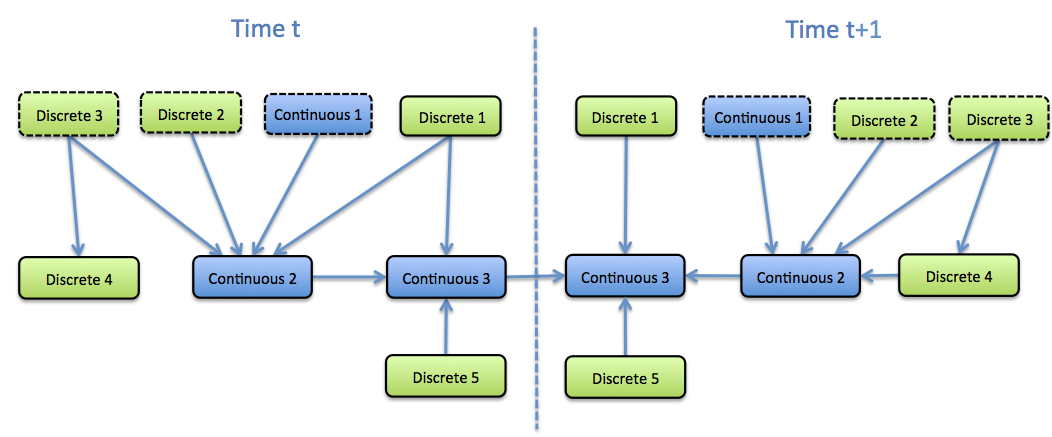
\includegraphics[scale=0.4]{./figures/AMIDSTModelClassLowPart}
%\caption{\label{Figure:AMIDSTModelClassHighLevel} AMIDST model class low part}
%\end{center}
%\end{figure}